\documentclass[10pt,a4paper]{cerndoc}

\usepackage{tikz-timing}


\CernDocSection{CERN BE-CO-HT}
\CernDocType{}
\CernDocTitle{Gennum GN4124 to Wishbone bridge }
\CernDocEditedBy{Simon Deprez}
\CernDocCheckedBy{Erik van der Bij}
\CernDocDate{May 2010}
\CernDocAbstract{Gennum is providing an IP core that can be used for hardware designs with the PCI express chip interface GN412x. This document describes how to extend the functionality to implement a simple wishbone master and shows its use in a simple test application.}
\lstset{
basicstyle=\normalsize\ttfamily,
frame=trBL,
morecomment=[l][\color{blue}]{--},
backgroundcolor=\color{yellow!20},
showstringspaces=false}

\begin{document}
\cerntitle
\section*{Revision History}
\begin{tabularx}{\textwidth}{|p{3cm}|p{3cm}|X|}
\hline \textbf{Version}&\textbf{Date}&\textbf{Notes}\\ \hline \hline
0.1 & 10-03-2010 & Created\\ \hline
0.2 & 01-03-2010 & First draft\\ \hline
0.2 & 14-04-2010 & Add Wishbone master description \\ \hline
%0.3 & 26-04-2010 & Add Makefile changes\\ \hline
0.4 & 27-04-2010 & Add Wishbone slave description\\ \hline
0.5 & 04-05-2010 & More about Wishbone master\\ \hline
0.6 & 04-05-2010 & Review + Linux\\ \hline
\end{tabularx}

\tableofcontents
\listoffigures
\clearpage

\section*{Introduction}
\addcontentsline{toc}{section}{Introduction}
This project aims to provide a Wishbone master generic interface for FMC\footnote{See \href{http://www.vita.com/fmc.html}{http://www.vita.com/fmc.html}.} projects controlled by a PCI express access.

The PCIe FMC carrier\footnote{See \href{http://www.ohwr.org/projects/fmc-pci-carrier}{http://www.ohwr.org/projects/fmc-pci-carrier}.} will be associated with several FMC mezzanines.

This file explains how to start with the GN4124 IP core. It describes the testbench environment provided by Gennum (Beta version) to simulate the IP. 

The Wishbone master is written as simple as possible

%%%%%%%%%%%%%%%%%%%%%%%%%%%%%%%%%%%%%%%%%%%%%%%%%%%%%%%%%%%%%%%%%%%%%%%%%%%%%%%%
%%%%%%%%%%%%%%%%%%%%%%%%%%%%%%%%%%%%%%%%%%%%%%%%%%%%%%%%%%%%%%%%%%%%%%%%%%%%%%%%
\section{Gennum IP core}
\subsection{Gennum documentation}

Gennum documentation files can be obtained from the following url: 

\texttt{http://my.gennum.com/mygennum/view.php/gn4124-gullwing}

A registration is required. The registration must be validated.

The reader is required to be acquainted with the following documentation:
\begin{itemize}
  \item GN412x PCI Express family Reference Manual (52624-0):
  \begin{itemize}
    \item Overview (p 11--12),
    \item Timing diagrams (p 41, 52--55),
    \item DMA core diagram (p 84);
  \end{itemize}
  
  \item GN412x FPGA IP Hardware Design Guide (51860-2):
  \begin{itemize}
    \item Overview (p 7),
    \item DMA sequencer limitations (p 9),
    \item DMA core diagram (p 22),
    \item Project register map (p 50);
  \end{itemize}
  \item GN412x RDK Software Design Guide (51859-1):
Describes the software furnished with the development kit;
  \item GN412x Simulation Test Bench User Guide (53716):
Tutorial for the simulation environment;
  \item GN412x BFM Reference Manual:
Describes the Bus Functional Model used for the Testbench.
\end{itemize}

The testbench zip archive (\verb+GN412x_TestBench_ModelSim(Beta_0.2.0).zip+) contains the last two documents.

\subsection{Gennum ISE project}

The Xilinx ISE project name is Lambo. The project must be migrated to a new version of Xilinx ISE. 
The project files can be obtained from the following url (a registration is required): 

\texttt{http://my.gennum.com/mygennum/view.php/gn4124-gullwing}. 

Select \verb+GN412x FPGA IP Xilinx Version 2009-05-26+.

After synthesis, the bitstream can be downloaded on the Gennum development kit with the \verb+gendiag+ program.

The \verb+gendiag+ program can be downloaded from the Gennum web site. 

Select \verb+ GN412x RDK SW 1.3 Windows+. A linux version is existing.

Edit the file \verb+C:\Program Files\GN412x_RDK\GenDiag\gendiag.ini+. The last lines contains the path of the Xilinx bitstream file :
\begin{lstlisting}
 <path>\lambo.bit
\end{lstlisting}

Run \verb+gendiag+.

\subsection{Linux Gendiag compilation}
Read the file \verb+./README+.

In the file \verb+./src/kdrv/Linux/uio.c+, add the folowing line (with Ubuntu):
\begin{lstlisting}
 #include <linux/sched.h>
\end{lstlisting}


%%%%%%%%%%%%%%%%%%%%%%%%%%%%%%%%%%%%%%%%%%%%%%%%%%%%%%%%%%%%%%%%%%%%%%%%%%%%%%%%
%%%%%%%%%%%%%%%%%%%%%%%%%%%%%%%%%%%%%%%%%%%%%%%%%%%%%%%%%%%%%%%%%%%%%%%%%%%%%%%%
\section{Wishbone master}

This project is based on the Gennum FlexDMA IP core.

Gennum IP provides a CSR interface similar to Wishbone but not totally compatible. There is no acknowledge that permit to slave to indicates normal termination of a bus cycle. There is no signal to differentiate read cycle of a wait state.

The DMA sequencer is driven with the original target controller interface. A modification of this interface implies the modification of the sequencer. A

  \subsection{Application Attachment layer modifications}
The Application attachment layer is the main part of the Gennum core. See Figure~\ref{fig:GCWWM}. It contains DMA masters and the target controller. A Wishbone master interface is added. This new interface transforms PCIe write into Wishbone write and a PCIe read into a Wishbone 'delayed' read. 

The \verb+./fpga_project/lambo/design/rtl/+ folder in the testbench environment contains all the Gennum IP files.

\begin{figure}[!ht]
	\centering
		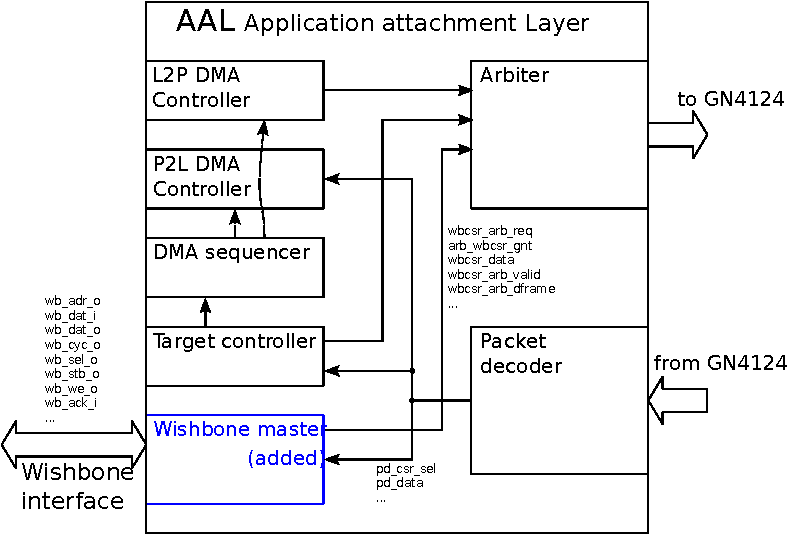
\includegraphics[width=\textwidth]{GennumCore}
	\caption{Gennum core with Wishbone master}
	\label{fig:GCWWM}
\end{figure} 





  
    \subsubsection{Arbiter}
Add an entry for \verb+wbmaster+ module. The file \verb+arb.v+ is modified to accept packets of the \verb+wbmaster+ module.
The added signals are :
\begin{itemize}
  \item\texttt{wbm\_arb\_data} : input;
  \item\texttt{wbm\_arb\_valid} : input;
  \item\texttt{wbm\_arb\_dframe} : input;
  \item\texttt{wbm\_arb\_req} : input; 
  \item\texttt{arb\_wbm\_gnt} : output.
  
\end{itemize}
    \subsubsection{Packet decoder}
The packet decoder (\verb+packet_decoder.v+) is not modified.
    
  \subsection{Wishbone master module}  
A Wishbone master based on Gennum Target module (\verb+tar.v+) is added. It supports single read and single write of 32 bit data.
The Wishbone bus clock frequency is 100 MHz. The Gennum FlexDMA local clock is used.
   
Addresses between 400h and 7FCh are routed to the wishbone master (see \verb+dma.v+). On the Wishbone bus the address range is 100h -- 1FFh for 32 bit registers. This can be redefined in the file \verb+dma.v+.  
    
Wishbone signals are added to the application attachment layer entity (\verb+dma.v+) :
\begin{itemize}
  \item\texttt{wb\_adr\_o} : output;
  \item\texttt{wb\_dat\_i} : input;
  \item\texttt{wb\_dat\_o} : output;
  \item\texttt{wb\_cyc\_o} : output;
  \item\texttt{wb\_sel\_o} : output;
  \item\texttt{wb\_stb\_o} : output;
  \item\texttt{wb\_we\_o} : output;
  \item\texttt{wb\_ack\_i} : input.
\end{itemize}     
   This signals are also present in \verb+wbmaster+ module and replace original target interface(see \verb+tar.v+).

\subsubsection{Wishbone master limitations}
    Data transfers are limited to single writes and single read.
    During a wishbone cycle, new requests are ignored.

\subsubsection{Write request} 
When a single write packet is addressed to the wishbone master, the module drive the wishbone bus signals (see figure \ref{fig:WR}). Then, the module wait for an acknowledge from a wishbone slave to terminate the cycle. During the wishbone cycle, the other PCIe requests are ignored. Wishbone cycles have a timeout of 7 clock cycles.
\begin{figure}[!ht]
	\centering

\begin{tikztimingtable}
  lclk                         & H29{C}                           \\
  pd\_csr\_sel                 & 2L 2H 10L 2H 14L                 \\
  pd\_data [31:0]              & 2U 2D{A0} 10U 2D{H1} 2D{D1} 12U  \\
  pd\_data [63:32]             & 2D{H0} 2D{D0} 10U 2D{A1} 14U     \\
  \\ % Gives vertical space
  wb\_adr\_o                   & 4D{0} 4D{A0} 10D{0} 4D{A1} 8D{0} \\
  wb\_dat\_o                   & 4D{0} 4D{D0} 10D{0} 4D{D1} 8D{0} \\
  wb\_cyc\_o                   & 4L 4H N(B) 0.1L N(C) 7.9L 6H 8L  \\
  wb\_sel\_o                   & 4D{0} 4D{F} 10D{0} 4D{F} 8D{0}   \\
  wb\_stb\_o                   & 4L 4H 10L 4H 8L                  \\
  wb\_we\_o                    & 4L 4H 10L 4H 8L                  \\
  wb\_ack\_i                   & 6L 0.1H N(A) 2.4H N(D) 11.5L 2.5H 7.5L     \\
  \extracode
  \draw[orange,semithick,->](A) .. controls +(right:0.5cm) and +(left:0.5cm) .. (B);
  \draw[orange,semithick,->](C) .. controls +(right:0.5cm) and +(left:0.5cm) .. (D);
\begin{pgfonlayer}{background}
\begin{scope}[gray,semitransparent,semithick]
\vertlines {2,4,...,29}
\end{scope}
\end{pgfonlayer}
\end{tikztimingtable}

	\caption{Write request}
	\label{fig:WR}
\end{figure} 

\subsubsection{Read request} 
The process is the same as for a write request but the write enable signal isn't asserted. When the wishbone cycle is terminated, a simple read completion packet is sent to the arbiter (see figure \ref{fig:RR}).


\begin{figure}[!ht]
	\centering

\begin{tikztimingtable}
  lclk                         & H29{C}                           \\
  pd\_csr\_sel                 & 2L 2H 10L 2H 14L                 \\
  pd\_data [31:0]              & 2U 2D{A0} 26U                    \\
  pd\_data [63:32]             & 2D{H0} 28U                       \\     
  \\ % Gives vertical space                                 
  wb\_adr\_o                   & 4D{0} 4D{A0} 22D{0}              \\
  wb\_dat\_i                   & 6U 2D{D0} 22U                    \\
  wb\_cyc\_o                   & 4L 4H 22L                        \\
  wb\_sel\_o                   & 4D{0} 4D{F} 22D{0}               \\
  wb\_stb\_o                   & 4L 4H 22L                        \\
  wb\_we\_o                    & 30L                              \\
  wb\_ack\_i                   & 6L 2.5H 21.5L                    \\
  \\ % Gives vertical space
  csr\_arb\_req                & 8L 4H 18L                        \\
  arb\_csr\_gnt                & 10L 4H 16L                       \\
  csr\_arb\_data[31:0]         & 10D{0} 2D{H0} 18D{0}             \\
  csr\_arb\_data[63:32]        & 10D{0} 2D{D0} 18D{0}             \\
  csr\_arb\_valid              & 10D{00} 2D{11} 18D{00}           \\
  csr\_arb\_dframe             & 10D{00} 2D{01} 18D{00}           \\
  \extracode
\begin{pgfonlayer}{background}
\begin{scope}[gray,semitransparent,semithick]
\vertlines {2,4,...,29}
\end{scope}
\end{pgfonlayer}
\end{tikztimingtable}
 
	\caption{Read request}
	\label{fig:RR}
\end{figure} 

\subsubsection{Wishbone datasheet} 

\begin{tabularx}{\textwidth}{|X|cc|}
\hline \multicolumn{3}{|c|}{WISHBONE DATASHEET for the 32-bit MASTER with 8-bit granularity}\\ \hline\hline
\multicolumn{1}{|c|}{Description} &\multicolumn{2}{c|} { Specification}                                 \\ \hline
General description                &\multicolumn{2}{l|} { Wishbone master controlled by PCI express}     \\ \hline
Supported cycles                   &\multicolumn{2}{l|} { MASTER, READ/WRITE }                           \\ \hline
Data port, size:                   &\multicolumn{2}{l|} { 32-bit}                                        \\
Data port, granularity:            &\multicolumn{2}{l|} { 8-bit}                                         \\
Data port, maximum operand size    &\multicolumn{2}{l|} { 32-bit}                                        \\
Data transfer ordering:            &\multicolumn{2}{l|} { Big endian and/or little endian}               \\
%Data transfer sequencing:          &\multicolumn{2}{l|} { Undefined}                                     \\ \hline
Clock frequency constraints:       &\multicolumn{2}{l|} { 100 MHz (Gennum IP local clock)}               \\ \hline
\multirow{8}{6cm}{Supported signal list and cross reference to equivalent WISHBONE signals}
&  Signal Name   & WISHBONE Equiv.                                                                        \\ %\hline
&  CLK\_O        &  CLK\_I                                                                                \\ %\hline
&  CYC\_O        &  CYC\_O                                                                                \\ %\hline
&  STB\_O        &  STB\_O                                                                                \\ %\hline
&  ADR\_O(10..0) &  ADR\_O()                                                                              \\ %\hline
&  DAT\_I(31..0) &  DAT\_I()                                                                              \\ %\hline
&  DAT\_O(31..0) &  DAT\_O()                                                                              \\ %\hline
&  WE\_O         &  WE\_O                                                                                 \\ %\hline
&  ACK\_I        &  ACK\_I                                                                                \\ %\hline
%Special requirements:              &\multicolumn{2}{p{8cm}||} { }                                         \\ 
\hline


\end{tabularx}

\clearpage   
  \subsection{Wishbone slave}  
A Wishbone slave module (\verb+wb_debug.vhd+) was generated with the CERN\verb+wbgen2+\footnote{See Wishbone slave generator: \href{http://www.ohwr.org/projects/wishbone-gen}{http://www.ohwr.org/projects/wishbone-gen}.} script with 3 registers of 8 bits for tests.
It was connected to debug leds and buttons of the gennum kit and to the wishbone master.   

The input description file for \verb+wbgen2+ is \verb+wb_debug.wb+ :
\begin{lstlisting}[basicstyle=\footnotesize\ttfamily]
-- here comes our peripheral definition
peripheral {
-- short (human-readable) name for the peripheral.
  name = "Gennum card debug Wishbone slave core";
-- a longer description, if you want
  description = "An 8-bit output port";
-- name of the target VHDL entity to be generated
  hdl_entity = "wb_gpio_debug";
-- prefix for all the generated ports belonging to our peripheral
  prefix = "gpio";

-- Ouput register
  reg {
    name = "LED port";
    description = "Output port";
    prefix = "led";
    field {
      name = "Port output value";
      description = "Reflects the state of LEDs.";
      type = SLV;
      size = 8;
      access_bus = READ_WRITE;
      access_dev = READ_ONLY;
    };
  };
		
  reg {
    name = "DEBUG port";
    description = "Input port";
    prefix = "debug";
    field {
      name = "Port input value";
      description = "Reflects the state of the DEBUG switch.";
      type = SLV;
      size = 8;
      access_bus = READ_ONLY;
      access_dev = WRITE_ONLY;
    };
  };
		
  reg {
    name = "Test register";
    description = "Test register";	
    prefix = "test";
    field {
      name = "Test register";
      description = "Test read and write register";
      type = SLV;
      size = 8;
      access_bus = READ_WRITE;
      access_dev = READ_ONLY;
    };
  };
};   
\end{lstlisting}   
   
%%%%%%%%%%%%%%%%%%%%%%%%%%%%%%%%%%%%%%%%%%%%%%%%%%%%%%%%%%%%%%%%%%%%%%%%%%%%%%%%
%%%%%%%%%%%%%%%%%%%%%%%%%%%%%%%%%%%%%%%%%%%%%%%%%%%%%%%%%%%%%%%%%%%%%%%%%%%%%%%%   
\section{DMA controller}
  \subsection{Gennum Pinto project}
This project contains a Xilinx DDR2 ram controller used for DMA transfer.

The project must be migrated to a new version of Xilinx ISE.
If the file \verb+C:\pinto\pinto.xcf+ cannot be found by the synthesizer, change the path by click-right on \verb+Synthesize - XST+ and choose \verb+Process properties+. Set the good path for the Synthesis Constraints File.
  

%%%%%%%%%%%%%%%%%%%%%%%%%%%%%%%%%%%%%%%%%%%%%%%%%%%%%%%%%%%%%%%%%%%%%%%%%%%%%%%%
%%%%%%%%%%%%%%%%%%%%%%%%%%%%%%%%%%%%%%%%%%%%%%%%%%%%%%%%%%%%%%%%%%%%%%%%%%%%%%%%
\section{Gennum Simulation Testbench}
  \subsection{Some issues}
    \subsubsection{Path error}
The file \verb+modelsim.ini+ contain an absolute path reference to the file \verb+vlog.opt+ at line 256.

Change the line to :
\begin{lstlisting}
 OptionFile = vlog.opt
\end{lstlisting}
	
    \subsubsection{Error with address in BFM scripting using C}
The \verb+long long int+ variables make errors in the format string of \verb+printf+ commands when the MinGW (Windows) compiler is used. 
In the address placeholders of the format string, the length parameter \verb+ll+ must be replaced by \verb+I64+.

Replace \verb+%016llX+
by \verb+%016I64X+ 
in the file \verb+./Test_Builder/lib/model.c+ at lines 64, 73, 288 and 298.


	\subsubsection{Testbench with Linux}
The names of the UNISIM library files are containing capitals letters. The Makefile uses small letter for this files.

In the \verb+.\unisims\+ folder, run the command ;
\begin{lstlisting}
 rename 'y/A-Z/a-z/' *
\end{lstlisting}


  \subsection{Makefile}
Rules are added for both Wishbone master \verb+wbmaster.v+ (line 51-53) and wishbone slave \verb+wb_gpio.vhd+ (line 49-51).

Dependencies are added in the top module (\verb+lambo.v+, line 45) rule in the Makefile.
	
	
  \subsection{BFM script}
Gennum provides a Testbench environment that emulates the local bus between the GN4124 chip and the FPGA. The Bus Functional Model is used to simulate PCI access for the FPGA system.
	
The file \verb+wbmaster_test.c+ contains a script with read and write requests for the wishbone bus.
  
  
  \subsection{Simulation}
Read the GN412x Simulation Test Bench User Guide (53716).

The file \verb+./Test_builder/wbmaster_test.c+ is a simple BFM script used for the testbench with the wishbone master.
 
Open a terminal and use the command :
\begin{lstlisting}
 test wbmaster_test
\end{lstlisting}

In Modelsim, run the simulation :
\begin{lstlisting}
 do lambo.do
\end{lstlisting}



  
    


\section*{Summary}
\addcontentsline{toc}{section}{Summary}
The modifications made to the files original from Gennum made possible to implement a Wishbone master that is simple and allows single read and single write cycles of 32 bit data.

\end{document}










